\chapter{数列的极限}

\section{数列的极限概念}
在前一章中,我们已经看到任何一个实数都可以用有理
数来左、右夹逼,即对于任何实数$x$我们总可以用逼近法求
得两个有理数列$\{a_n\}$, $\{b_n\}$使得
\[a_1\le a_2\le \cdots \le a_n\le \cdots\le x\le \cdots\le b_n\le \cdots\le b_2\le b_1\]
并且$b_n-a_n$可以小到任意小。

数列中的项$a_n$和$b_n$就是$x$的第$n$次不足近似值和过剩近似
值,它们的误差可以用不等式
\[|x-a_n|<b_n-a_n,\qquad |x-b_n|<b_n-a_n\]
来估计。这里所说的逼近的要点在于\textbf{误差可以小到任意小},
下面用例子从另一个角度来说明这一点。

今以$\frac{2}{3}$为例,作上述分析:
\begin{enumerate}
    \item 以3去除2,得:
    \begin{center}
  \longdivision[2]{2.00}{3}      
    \end{center}
    因为每次20除以3都余2, 所以商数6重复出现,这个
    除法可以无止境地作下去。
    \item 上述除式的意义是
\[\begin{split}
    2&=0.6\x3+0.2\Longleftrightarrow 0.6<
\frac{2}{3}<0.7,\\
&=0.66\x3+0.02\Longleftrightarrow 0.66<
\frac{2}{3}<0.67,\\
&=0.666\x3+0.002\Longleftrightarrow 0.666<
\frac{2}{3}<0.667,\\
\cdots &\cdots\cdots\cdots\cdots\cdots\cdots\cdots
\end{split}\]
\end{enumerate}

从上面的分析,同学们可以看出$\frac{2}{3}$
显然不能用有限位
小数表示出,但是存在着由有限位小数所成的无穷数列$\{a_n\}$
和$\{b_n\}$
\[\begin{split}
    \{a_n\}&:\quad a_1=0.6,\; a_2=0.66,\; a_3=0.666,\; \ldots ,\; a_n=0.\underbrace{66\cdots66}_{\text{$n$位小数}},\; \ldots\\
    \{b_n\}&:\quad b_1=0.7,\; b_2=0.67,\; b_3=0.667,\; \ldots ,\; b_n=0.\underbrace{66\cdots67}_{\text{$n$位小数}},\; \ldots
\end{split}\]
满足 
\[a_n=0.\underbrace{66\cdots66}_{\text{$n$位小数}}<\frac{2}{3}<0.\underbrace{66\cdots67}_{\text{$n$位小数}}=a_n+\frac{1}{10^n}\]
并且$a_n$与$\frac{2}{3}$
之间的误差
$\left|a_n-\frac{2}{3}\right|<b_n-a_n=\frac{1}{10^n}$, 同样
$b_n$与$\frac{2}{3}$之间误差$\left|b_n-\frac{2}{3}\right|<\frac{1}{10^n}$,只要$n$充分大,误差
可以小到任意小。上面的逼近过程,表明无穷数列$\{a_n\}$, $\{b_n\}$从左、右两方面趋近$\frac{2}{3}$,可以使其误差任意小,$\frac{2}{3}$就是数列$\{a_n\}$的极限,也是数列$\{b_n\}$的极限,用符号表示就是
\[\lim_{n\to\infty}a_n=\frac{2}{3},\qquad \lim_{n\to\infty}b_n=\frac{2}{3}\]
或者用
\[a_n\to \frac{2}{3},\qquad b_n\to\frac{2}{3},\qquad a_n\to \frac{2}{3}\leftarrow b_n\]
来生动地表述上述事实。

从这里我们看到逼近与极限是密切相关的,极限只是把
逼近过程推进到无穷$(n\to\infty)$的结果,逼近只要误差小到
所要求的精确度后就可以停止。$\Lim_{n\to\infty}a_n=\frac{2}{3}$
表示数列$\{a_n\}$当
$n$无限增大的极限值是$\frac{2}{3}$。

我们再用极限的观点对$\sqrt{2}$ 进行分析如下。$\sqrt{2}$是一
个什么数?要回答这个问题,我们只须找出有理数
$\frac{a}{b}$
在什么时候大于$\sqrt{2}$, 什么时候小于$\sqrt{2}$, 也就是说,如果
$\left(\frac{a}{b}\right)^2<2$, 那么正数$\frac{a}{b}<\sqrt{2}$;如果$\left(\frac{a}{b}\right)^2>2$, 那么
$\frac{a}{b}>\sqrt{2}$. 根据有理数是有序的,稠密的,因此有理数的
平方总能和2比较大小,这就保证我们可以用逼近法(譬如
十分逼近法)决定左、右夹逼$\sqrt{2}$的两个由十进位小数组
成的数列$\{a_n\}$、$\{b_n\}$如下:
\[\begin{split}
    \{a_n\}&:\quad a_1=1,\; a_2=1.4,\; a_3=1.41,\; a_4=1.414,\ldots\\
    \{b_n\}&:\quad b_1=2,\; b_2=1.5,\; b_3=1.42,\; b_4=1.415,\ldots\\
\end{split}\]
使得$a_n<\sqrt{2}<b_n$, 而且$b_n-a_n=\frac{1}{10^n}$,
于是
\[|a_n-\sqrt{2}|<\frac{1}{10^n},\qquad |b_n-\sqrt{2}|<\frac{1}{10^n} \]
这就是说,第$n$次的有限小数近似值$a_n$和$b_n$与$\sqrt{2}$的误
差分别小于$\frac{1}{10^n}$,
因此,只要$n$充分大,误差就可以小到任
意小,当我们让这个计算过程,无穷地进行下去时,我们就
说$\sqrt{2}$ 是数列$\{a_n\}$或$\{b_n\}$的极限,记做
\[\lim_{n\to\infty}a_n=\sqrt{2},\qquad \lim_{n\to\infty}b_n=\sqrt{2}\]

从上面两个例子看到,实数是具有$n$位数字的普通十进
位小数数列,当$n$无限增大时的极限。

如今我们说明了逼近与极限概念密切相关的一面,但是
极限与逼近也有观点不同,概念层次也不同的方面,上面所
说用十分逼近法求$\sqrt{2}$ 的近似值$1,1.4,1.41,\ldots$等是逼
近的观点,它是先有$\sqrt{2}$ ,即我们先知道$\sqrt{2}$  是方程$x^2=2$
的根,然后用小数去逐步逼近。极限的观点恰恰相反,它是
先有一个无穷数列$\{a_n\}$,然后要去看一下,它们是否恰好无
限逼近某一个常数$A$. 假如是这样,就叫$A$是数列$\{a_n\}$的极
限值。

下面介绍几个逼近某一常数的无穷数列的例子。

\begin{example}
    仔细观察数列:
    \[1,\; \frac{1}{2},\;\frac{1}{3},\;\frac{1}{4},\; \ldots,\;\frac{1}{n},\;\ldots\]
我们马上看出
\begin{enumerate}
    \item 上述数列的每一项都是正数。
    \item 上述数列逐项递减:
\[1>\frac{1}{2}>\frac{1}{3}>\cdots>\frac{1}{n}>\frac{1}{n+1}>\cdots>0\]
因而是一个递减有界数列。
\item 当$n$愈来愈大时,$a_n=\frac{1}{n}$
愈来愈接近0, 它们的
误差$|a_n-0|=\frac{1}{n}$, 只要充分大,就可以小到任意小。
\end{enumerate}

对于情形3,我们就说:数列$\left\{\frac{1}{n}\right\}$
趋近于0或收敛到0, 或0是数列$\left\{\frac{1}{n}\right\}$
的极限,并记作$\frac{1}{n}\to 0$
或$\Lim_{n\to\infty}\frac{1}{n}=0$。

现在,让我们再用数轴把上述事实图解说明如下:
\begin{figure}[htp]
    \centering
    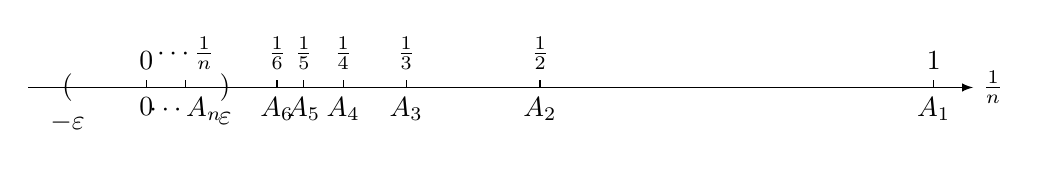
\begin{tikzpicture}[>=latex]
 \draw[->] (-1.5,0)--(10.5,0)node[right]{$\frac{1}{n}$};
\foreach \x/\xtext in {1/A_1,.5/A_2,.33/A_3,.25/A_4,.2/A_5,.166/A_6,0/0}
{
    \draw (\x*10,0)node[below]{$\xtext$}--(\x*10,.1);
}
\foreach \x/\xtext in {1/1,.5/\frac{1}{2},.33/\frac{1}{3},.25/\frac{1}{4},.2/\frac{1}{5},.166/\frac{1}{6},0/0}
{
    \node at (\x*10,.1)[above]{$\xtext$};
}
\node at (-1,0){(};
\node at (1,0){)};
\node at (-1,-.2)[below]{$-\varepsilon$};
\node at (1,-.2)[below]{$\varepsilon$};
\draw (.5,0)node[below]{$\cdots A_n$}--(.5,.1)node[above]{$\cdots \frac{1}{n}$};
    \end{tikzpicture}
    \caption{}
\end{figure}

在数轴上取以数列:
\[1,\; \frac{1}{2},\;\frac{1}{3},\;\frac{1}{4},\; \ldots,\;\frac{1}{n},\;\ldots\]
的各项为坐标的各点,就得到一个点列:
\[A_1,A_2,A_3,A_4,\ldots,A_n,\ldots,\]
上述点列$\{A_n\}$从原点$O$的右边逐步向原点逼近,而且点$A_n$到
原点的距离$|a_n-0|=\frac{1}{n}$,
只要$n$充分大,就可以小到任
意小。上面的事实也可以这样来说明:通常我们把$A$点为中
心的\textbf{开区间}$(A-\varepsilon,A+\varepsilon)$叫做这\textbf{点$A$的$\varepsilon$邻域}。我们看到,
原点$O$的任意$\varepsilon$邻域,包
含$\left\{\frac{1}{n}\right\}$
的除有限个点以外的全部
点。这也就是说数列$\left\{\frac{1}{n}\right\}$
是收敛的,并且收敛到0。
\end{example}

\begin{example}
观察数列$\left\{\frac{n}{n+1}\right\}: \frac{1}{2},\frac{2}{3},\ldots,\frac{n}{n+1},\ldots$
同学们容易看出,这个数列逐项递增,其各项$a_n=\frac{n}{n+1}$
永
远小于1, $a_n$和1之间的误差$|a_n-1|=\left|\frac{-1}{n+1}\right|=\frac{1}{n+1}$,
只要$n$充分大就可以到任意小。这也就是说,这个数列在
数轴上的对应点列,除有限个点外全部点都在点1的 任意$\varepsilon$
邻域内(图3.2),因此,这个数列$\left\{\frac{n}{n+1}\right\}$
的极限是1, 或
者变量$a_n=\frac{n}{n+1}$
的极限是1, 用符号表示就是:
\[\frac{n}{n+1}\to 1,\quad \text{或者}\quad \lim_{n\to\infty}\frac{n}{n+1}=1\]
\begin{figure}[htp]
    \centering
\begin{tikzpicture}[>=latex]
\draw[->] (-.5,0)--(10,0)node[right]{$\frac{n}{n+1}$};
\foreach \x/\xtext in {0/0,.5/\frac{1}{2},.667/\frac{2}{3},.75/\frac{3}{4}, .8/\frac{4}{5},1/1}
{
    \draw (\x*8,0)node[below]{$\xtext$}--(\x*8,.1);
}
\node at (7+.3,0.2)[above]{$1-\varepsilon$};
\node at (9-.3,0.2)[above]{$1+\varepsilon$};
\node at (7+.3,0){(};
\node at (9-.3,0){)};

\end{tikzpicture}  
    \caption{}
\end{figure}
\end{example}

\begin{example}
    观察数列$\left(-\frac{1}{2}\right),\; \left(-\frac{1}{2}\right)^2,\; \left(-\frac{1}{2}\right)^3,\ldots,\left(-\frac{1}{2}\right)^n,\;\ldots$, 这个数列逐项正负相间,是摆动数列,显然,
    各项的绝对值$|a_n|\le\frac{1}{2}$, $n=1,2,3,\ldots$,因此,它又
    是有界的。其第$n$项与数0之间的误差$|a_n-0|=\left(\frac{1}{2}\right)^n$,当$n$充分大时,可以小到任意小。再从数轴上看,其对应点列从
    原点的左、右两侧向原点逼近,而且当$n$充分大时,$a_n$全部
    都在原点的任意$\varepsilon$邻域内(图7.3),因此,这个数列
$\left\{\left(-\frac{1}{2}\right)^n\right\}$的极限是0。
\begin{figure}[htp]
    \centering
 \begin{tikzpicture}[>=latex]
\draw[->] (-5.5,0)--(5.5,0)node[right]{$\left(-\frac{1}{2}\right)^n$};
\foreach \x/\xtext in {0/0,-1/-1,-.5/-\frac{1}{2},.25/\frac{1}{4},1/1}
{
    \draw (\x*5,0)node[below]{$\xtext$}--(\x*5,.1);
}
\foreach \x/\xtext in {0/{},-1/{},-.5/A_1,.25/A_2,1/{}}
{
    \node at (\x*5,.1)[above]{$\xtext$};
}

\foreach \x/\xtext in {-.125/A_3,.0625/A_4}
{
    \draw (\x*5,0)--(\x*5,.1)node[above]{$\xtext$};
}

\foreach \x/\xtext in {-.15/-\varepsilon,.15/\varepsilon}
{
    \node at (\x*5,-.15)[below]{$\xtext$};
}
\node at (-.75,0){(};
\node at (.75,0){)};


 \end{tikzpicture}   
    \caption{}
\end{figure}
\end{example}

从以上三个数列,我们看到它们的共性是在项数$n$无限
增大的过程中,参与在这个过程的变量$a_n=\frac{1}{n}$, $a_n=\frac{n}{n+1}$, 
$a_n=\left(-\frac{1}{2}\right)^n$
所取的值与某一个常数$A$的差的绝对值$|a_n-
A|$(或者说它们之间的绝对误差),只要$n$充分大,就可
以小到任意小。它们在数轴上对应的点列,只要$n$充分大,
除有限个点外全部点都在点$A$的任意$\varepsilon$邻域内。

让我们把只要$n$充分大,误差可以任意小的含义说得更
精确些。为此,再以例7.3说明之,我们来看它的第$n$项与0
的误差:
\[|a_n-0|=\left|\left(-\frac{1}{2}\right)^n-0\right|=\left(\frac{1}{2}\right)^n\]

当$n$为何值时,$\left(\frac{1}{2}\right)^n<0.0001$。解之,得
\[n\lg\left(\frac{1}{2}\right)<-4,\quad \text{即}\quad (-0.3010)n<-4\]
$\therefore\quad n>13.289$

因此,只须$n\ge 14$, 就有
\[|a_n-0|=\left(\frac{1}{2}\right)^n\le \left(\frac{1}{2}\right)^{14}=0.000061<0.0001\]
这也就是说,对于给定的0.0001, 总能找到这样一个项数,
$N=14$, 使得当$n\ge14$时,其误差
\[|a_n-0|=\left(\frac{1}{2}\right)^{14}<0.0001\]

当$n$为何值时,$\left(\frac{1}{2}\right)^n<\frac{1}{10^8}$
只须,
\[n\lg\left(\frac{1}{2}\right)<-8\]
即
\[n>\frac{-8}{-0.3010}=26.578\]
因此,只须$n\ge 27$时,就有
\[\left(\frac{1}{2}\right)^n<\left(\frac{1}{2}\right)^{27}=0.000000007=7\x 10^{-9}<10^{-8}\]

一般地,任给$\varepsilon >0$, 当$n$为何值时,$\left(\frac{1}{2}\right)^n<\varepsilon$。只须
\[n\lg \frac{1}{2}<\lg\varepsilon\] 
即
\[n>\frac{\lg\varepsilon}{-0.3010}\]
由于$\varepsilon$ 是任意小的正数,当$\varepsilon <1$时,$\lg\varepsilon <0$。于是
$\frac{\lg\varepsilon}{-0.3010}$
是正数,因此,我们总能找到这样项数$N=\left(\frac{\lg\varepsilon}{-0.3010}\text{的整数部分}\right)+1$
,使得当$n\ge N$,
\[|a_n-0|=\left(\frac{1}{2}\right)^n<\left(\frac{1}{2}\right)^N<\varepsilon  \]

现在,我们可以给数列$\{a_n\}$的极限是$A$以精确定义
如下:

\begin{blk}{定义}
    任给正数$\varepsilon$, 总可以定出一个正整数$N$, 使得只
要$n\ge N$时,$|a_n-A|<\varepsilon$都成立,我们就说数列$\{a_n\}$的\textbf{极限
是}A, 或者说数列$\{a_n\}$\textbf{收敛到}$A$。
\end{blk}
 
让我们再对上述定义作几点说明:
\begin{enumerate}
\item $\varepsilon$ (读成Epsilon)是希腊字母,相当于英文字母
的$e$, 它是error(误差)的头一个字母,误差任意小的数
量提法就是“小于任给正数$\varepsilon$”。
\item $a_n$是逐步逼近$A$的,要使误差$|a_n-A|$愈小(或者
说够小)那就要让数列的项数$n$变得够大,所以“只要$n\ge
N$时,$|a_n-A|<\varepsilon$ ”的意义也就是:“只要$n$够大,误差$|a_n
-A|$就会小到所要求的那么小!”
\item $\varepsilon$是任给的正数,是变量,但是当误差范围$\varepsilon$一经
给定之后,就为常数,我们对于这个指定的$\varepsilon$检验是否存在
具有上述性质的$N$, 在求$N$的过程中,$\varepsilon$的值不能变动,一般
说来,给的$\varepsilon$愈小,那么求得的$N$愈大。
\item 定义中的当$n\ge N$时,$|a_n-A|<\varepsilon$等价于当$n\ge N$
时,$A-\varepsilon<a_n<A+\varepsilon$或$a_n\in (A-\varepsilon,A+\varepsilon)$, 这就是说,如
果数列$\{a_n\}$收敛于$A$则在点$A$的任何$\varepsilon$邻域内必包含这个数列
的除有限个项以外的一切项。
\end{enumerate}


为了帮助同学熟悉极限定义,我们在下面再举几个例
子,说明$N$的大小和$\varepsilon$之间的关联,并给出证明某数是已
知数列的极限的方法。

\begin{example}
    证明数列$\left\{\frac{n}{n+1}\right\}$
的极限是1。
\end{example}

\begin{solution}
对于任给$\varepsilon>0$,要使
\[\left|\frac{n}{n+1}-1\right|=\frac{1}{n+1}<\varepsilon\]
只须$n+1>\frac{1}{\varepsilon}$,即$n>\frac{1}{\varepsilon}-1$,取$N=\left(\frac{1}{\varepsilon}-1\right)$
的整数部分$+1$,所以当$n\ge N$时,可使
\[\left|\frac{n}{n+1}-1\right|=\frac{1}{n+1}\le \frac{1}{N+1}<\varepsilon\]
    这就是说$\Lim_{n\to\infty}\frac{n}{n+1}=1$。
\end{solution}

\begin{example}
    证明数列:
$1,0,\frac{1}{2},0,\frac{1}{3},0,\ldots,0,\frac{1}{n},0,\ldots$的极
限是0。
\end{example}

\begin{proof}
  这个数列的通项公式可以写成
\[a_n=\begin{cases}
    0,& \text{当$n$为偶数时;}\\
   \frac{2}{n+1},& \text{当$n$为奇数时。}
\end{cases}\]

对于任给$\varepsilon>0$, 因为数列$\{a_n\}$的所有偶数项为0, 所
以从第二项开始以后的所有偶数项都小于给定的$\varepsilon$. 现在须
从奇数项中确定从哪一项开始以后的一切项与0的误差小
于$\varepsilon$. 

令奇数项与0的误差:$\frac{2}{n+1}<\varepsilon$,即
\[n+1>\frac{2}{\varepsilon},\qquad n>\frac{2}{\varepsilon}-1\]  
取$N=\left(\frac{2}{\varepsilon}-1\right)$的整数部分加1,于是,当$n\ge N$,可使$\frac{2}{n+1}<\varepsilon$。所以对于任给$\varepsilon>0$, 从第$N$项开始以后的一切项都能使
$|a_n-0|<\varepsilon$
成立。即$\Lim_{n\to\infty}a_n=0$。
\end{proof}


\begin{example}
    证明数列$\left\{\frac{n^2-1}{n^2+n+1}\right\}$的极限是1。
\end{example}

\begin{proof}
对于任给$\varepsilon>0$, 
要使
\[|a_n-1|=\left|\frac{n^2-1}{n^2+n+1}-1\right|=\left|\frac{-n-2}{n^2+n+1}\right|=\frac{n+2}{n^2+n+1}<\varepsilon\]
看看是否存在这样的$N$, 使得当$n\ge N$时,永远有$|a_n-1|<\varepsilon$,
可是直接从上面的不等式解出$N$是不容易的,但我们
注意到,当$n$充分大时,在分子中起主导作用的是$n$, 而在
分母中起主导作用$n^2$. 如果把分子扩大为$2n\; (n>2)$, 又
把分母缩小为$n^2$, 这样有
\[|a_n-1|=\frac{n+2}{n^2+n+1}<\frac{2n}{n^2}=\frac{2}{n}\]

现在令$|a_n-1|<\frac{2}{n}<\varepsilon$,即$n>\frac{2}{\varepsilon}$,取$N$为$\frac{2}{\varepsilon}$的整数部分加1, 于是,当$n\ge N$时,可使
\[|a_n-1|>\frac{2}{n}<\varepsilon\]
这就是说$\Lim_{n\to\infty}\frac{n^2-1}{n^2+n+1}=1$。
\end{proof}

在上面的证明中,所取得的$N$比实际所需要的要大一
些,这样并不影响我们所要说明的问题:“$N$是根据预先给
定的$\varepsilon$来确定的,而且这个$N$满足极限定义中的条件”,事
实上,$N$不是由$\varepsilon$唯一确定的,对于给定的$\varepsilon>0$, 如果某
数,譬如10000可以充当极限定义中的$N$, 则大于10000的任
何一个自然数也都可以充当$N$, 自然$N$愈小愈好,但是,有时
候为了便于证明,不妨把$N$取得大些。问题的关键是是否存在
这样的$N$, 至于这个$N$是否是最小的,那是第二位的问题。

\begin{example}
说明数列$\left\{\sin^{2n}\frac{n\pi}{2}\right\}$没有极限。
\end{example}

\begin{proof}
这个数列各项的数值为
$1,0,1,0,\ldots$。
显然,1和0都不是这个数列的极限,因为在点1的小于1
的任何邻域之外,有此数列无穷多个数值为0的偶数项,同
样,在点0的小于1的任何邻域之外,有此数列无穷多个值
为1的奇数项。假设数$A\ne 0,1$并且是此数列的极限,则在
点$A$的任何$\varepsilon$邻域$(A-\varepsilon ,A+\varepsilon )$内都包含数0和1, 于是
\[2\varepsilon =(A+\varepsilon )-(A-\varepsilon )|>|1-0|=1\]
即:$\varepsilon>\frac{1}{2}$。
这和$\varepsilon$ 是任意小的正数矛盾,因此,这个数列没有极限。
\end{proof}

现在我们再来说明趋近于0的变量与收敛于某一个不等
于0的常数的变量之间的关系。从前面的例7.2和例7.6, 我们
看到当一个给定数列$\{a_n\}$的极限看出来等于$A\; (A\ne 0)$时,
我们需要验证的是$(a_n-A)\to 0$. 这个事实就是变量$a_n\to A\ne 0$
的必要充分条件是$(a_n-A)\to 0$.再者$a_n\to 0$的必要充分条
件是$|a_n|\to 0$。

前面所举的数列的例子,除例7.7之外,都有极限,我们已
经把这样的数列叫做\textbf{收敛数列}。如果数列不收敛就叫做\textbf{发散
数列}。显然无界数列是发散数列。下面给出一些发散数列的
例子。

对于一个数列$\{a_n\}$, 无论给出多么大的正数$M$, 都能找
到正整数$N$, 使得当$n\ge N$时,常有
$|a_n|>M$, 
我们说数列是\textbf{无限增大}的。

例如,$\{n^2\}$, $\{-n^2\}$, $\{(-n)\}$等数列都是无限增大的。

如果数列$\{a_n\}$是无限增大的,并且从某项以后的一切
项为正数时,我们说数列$\{a_n\}$趋于正无穷大,记作$\Lim_{n\to\infty}a_n=+\infty$,例如$\Lim_{n\to\infty}n^2=+\infty$。

如果数列$\{a_n\}$是无限增大的,并且从某项以后的一切
项为负数时,我们说数列$\{a_n\}$趋于负无穷大,记作$\Lim_{n\to\infty}a_n=-\infty$. 例如$\Lim_{n\to\infty}(-n^2)=-\infty$。

在无界数列中,也有不是无限增大的,例如,数列
\[\left(n\sin\frac{n\pi}{2}\right):\quad 1,0,-3,0,5,0,-7,0,\ldots\]
是无界的,但不是无限增大的,因为它的偶数项永远等
于0。

有界数列中也有发散的,例如前面例7.7的数列在两个数
值0和1上摆动。

\begin{blk}{命题}
    如果各项不为0的数列$\{a_n\}$是无限增大的,那么
它的倒数$b_n=\frac{1}{a_n}$
就组成以0为极限的数列;反过来,如果
各项不为0的数列$\{a_n\}$收敛到0, 那么它的倒数$b_n=\frac{1}{a_n}$就
组成无限增大的数列。
\end{blk}
 
事实上,对于任意给出的无论多么小的正数$\varepsilon$, 令$M=\frac{1}{\varepsilon}$
,根据数列$\{a_n\}$是无限增大的,一定可以找到正整数$N$, 使
得当$n\ge N$时,有$|a_n|>M$
成立,从而
\[|b_n|=\left|\frac{1}{a_n}\right|=\frac{1}{|a_n|}<\frac{1}{M}=\varepsilon\]
这就是说,
$\Lim_{n\to\infty}b_n=\Lim_{n\to\infty}\frac{1}{a_n}=0$。
同样也可以证明逆命题。

\section*{习题7.1}
\addcontentsline{toc}{subsection}{习题7.1}

\begin{enumerate}
    \item 数列的通项公式是
\[a_n=\frac{1000[1+(-1)^n]}{n},\quad n=1,2,3,\ldots,n,\ldots\]
\begin{enumerate}
    \item 计算这个数列的前5项,在数轴上图示这些
    数值;
    \item 对于$\varepsilon=1,\; 0.1,\; 0.01,\; 0.0001,\; 0.0000001$, 求
    出项数$N$, 使得当$n\ge N$时,$|ax|<1$, $|a_n|<0.1$, $|a_n|<0.01$, $|a_n|<0.0001$, $|an|<0.0000001$;
    \item 证明这个数列的极限为0。
\end{enumerate}

    \item 按定义证明下面数列的极限为0。
\begin{multicols}{2}
\begin{enumerate}
    \item $\left\{\frac{n+1}{n^2+1}\right\}$
    \item $\left\{\frac{\sin n}{n}\right\}$
    \item $\left\{\frac{1+2+3+\cdots+n}{n^3}\right\}$
    \item $\left\{\frac{1}{2\sqrt{n}}\right\}$
    \item $\left\{\frac{1}{n}+\frac{(-1)^n}{n^2}\right\}$
\end{enumerate}
\end{multicols}
    \item 证明数列:$0.9,\;0.99,\;0.999,\;\ldots$的极限是1.

    \item 证明$\frac{3n^5}{n^5-n^2+1}\to 3$.
    \item 说出下面数列的变化趋向:
\begin{multicols}{2}
\begin{enumerate}
    \item $\left\{\frac{100-3n}{100}\right\}$
    \item $\left\{(-1)^n\left(\frac{n-1}{n+1}\right)^2\right\}$
    \item $\left\{(-1)^n\frac{n^2+1}{n}\right\}$
    \item $\left\{\frac{1-(-1)^n}{2}n\right\}$
    \item $\left\{3(-1)^n+5\right\}$
    \item $\left\{n-(-1)^n\right\}$
\end{enumerate}
\end{multicols}
\end{enumerate}

\section{具有极限的数列的性质}
数列趋向于它们的极限时,有种种不同方式,例如在
例7.1中,数列$\left\{\frac{1}{n}\right\}$
趋向于它的极限时,不断地减小;在
例7.2中,数列
$\left\{\frac{n}{n+1}\right\}$趋向它的极限时,不断地增大,在例7.3中,数
列$\left\{\left(-\frac{1}{2}\right)^n\right\}$
趋向于它的极限时,时而增大,
时而减小,从极限值的两侧趋向于极限值0。

虽然数列趋向于它们各自的极限时,有各种不同的状
态,但是所有这些数列都具有一系列的共同的性质,我们现
在就来研究其中若干重要性质。

\begin{blk}{定理1}
     若$\Lim_{n\to\infty}a_n=A$, 而$A>p$(或$A<p$), 则存在数$N$, 当$n\ge N$时,永远有$a_n>p$(或$a_n<p$)。
\end{blk}

\begin{proof}
$\because\quad \Lim_{n\to\infty}a_n=A$
让我们取定正数$\varepsilon<A-p$ (或$p-A$), 从而
$$A-\varepsilon>p$$
根据数列极限定义,可以找到这样的$N$, 使得当$n\ge N$
时,有
$$A-\varepsilon<a_n<A+\varepsilon$$
于是,当$n\ge N$时,就有
$a_n>p$ (或$a_n<p$)。    
\end{proof}

定理1说明如果数列的极限大于(或小于)某一个实数,那
么收敛到此极限的数列从某一项起也大于(或小于)这个实
数。这个性质反映了收敛的数列和极限之间的密切关系。

\begin{blk}{定理2}
若$\Lim_{n\to\infty}a_n=A$, 而且当$n\ge N$时,$a_n\le p$ (或$a_n\ge p$),则$A\le p$ (或$A\ge p$)。
\end{blk}

\begin{proof}
 假设$A>p$, 根据定理1, 当$n\ge N$时,可使$a_n>
p$, 这与$a_n\le p$矛盾。

$\therefore\quad A\le p$。
\end{proof}

从例7.2看到$a_n=\frac{n}{n+1}<1$, 而$\Lim_{n\to\infty}\frac{n}{n+1}=1$. 这个例子说明从严格的不等式$a_n<p$和$\Lim_{n\to\infty}a_n=A$, 不能推出严
格的不等式$A<p$. 而定理2是说取极限过程使不大于或不
小于关系保持不变。

\begin{blk}{定理3}
    若$\Lim_{n\to\infty}a_n=A$, 则$A$是唯一的。
\end{blk}

\begin{proof}
用反证法,假设$a_n\to A$和$a_n\to B$且$A<B$, 在$A$与
$B$之间任取一数$R$, 设$A<R<B$, 因为$a_n\to A$, 且$A<R$,
所以可以找到$N_1$, 使得当$n\ge N_1$时,有$a_n<R$。

另一方面,$a_n\to B$, 且$B>R$, 所以可以找到$N_2$, 使得
当$n\ge N_2$时,有$a_n>R$。

取$N$为$N_1$和$N_2$中较大者,即$N=\max(N_1,N_2)$, 则当
$n\ge N$时,就有$a_n<R$, 同时又有$a_n>R$, 这是不可能的,因
此,数列的极限是唯一的。
\end{proof}

\begin{blk}{定理4}
    若$\Lim_{n\to\infty}a_n=A$, 则数列$\{a_n\}$是有界的。
\end{blk}    

\begin{proof}
由极限定义知,对于任意小正数$\varepsilon$, 可以找到$N$,
使得当$n\ge N$时,有
$A-\varepsilon<a_n<A+\varepsilon$。

设$A-\varepsilon,a_1,a_2,\ldots,a_N,A+\varepsilon$中最大的绝对值为$M$, 
则有$|a_n|\le M$,即数列$\{a_n\}$是有界的。
\end{proof}

\begin{blk}{定理5}
    若三个数列$\{a_n\},\{b_n\},\{c_n\}$的对应项满足不
等式$a_n<b_n<c_n$, 对于一切$n=1,2,3,\ldots$并且$\Lim_{n\to\infty}a_n=\Lim_{n\to\infty}c_n=A$,
则$\Lim_{n\to\infty}b_n=A$。
\end{blk}

\begin{proof}
\[\because\quad \Lim_{n\to\infty}a_n=A,\quad \Lim_{n\to\infty}c_n=A\]
根据数列极限定义知,对于任意给定$\varepsilon >0$, 存在正整数$N_1$,
使得当$n\ge N_1$时,有
\[A-\varepsilon <a_n<A+\varepsilon\] 
并且也存在一个正整数$N_2$, 使得当$n\ge N_2$, 有
\[A-\varepsilon <c_n<A+\varepsilon\]
令 $N=\max(N_1,N_2)$, 于是当$n\ge N$时,就同时有
\[A-\varepsilon <a_n<A+\varepsilon ,\qquad A-\varepsilon <c_n<A+\varepsilon \]
$\because\quad a_n\le b_n\le c_n,\quad n=1,2,3,\ldots$

$\therefore\quad $当$n\ge N$时,就有
\[A-\varepsilon <a_n\le b_n\le c_n<A+\varepsilon\]

这就是说,$\Lim_{n\to\infty}b_n=A$。
\end{proof}

定理5不仅告诉我们判断$\{b_n\}$的极限存在的一种方法,
而且也可用这方法来求极限。用这个方法,我们可以不去直接
求$\{b_n\}$的极限,而是把它和另外两个我们熟悉的有相同极限
的数列作比较。

\begin{example}
    求$\Lim_{n\to\infty}\frac{1}{n\left(\cos^2\frac{1}{2}n\pi+n\sin^2\frac{1}{2}n\pi\right)}$
\end{example}

\begin{solution}
\[\begin{split}
    \text{分母}&=n\left(\cos^2\frac{1}{2}n\pi+n\sin^2\frac{1}{2}n\pi\right)\\
    &=n\left[1+(n-1)\sin^2\frac{1}{2}n\pi\right]
\end{split}\]
又因为 $0\le \sin^2\frac{1}{2}n\pi\le 1$,所以
\[0<n\le n\left(\cos^2\frac{1}{2}n\pi+n\sin^2\frac{1}{2}n\pi\right)\le n^2\]
即
\[\frac{1}{n^2}\le \frac{1}{n\left(\cos^2\frac{1}{2}n\pi+n\sin^2\frac{1}{2}n\pi\right)}\le \frac{1}{n}\]
此外,$\Lim_{n\to\infty}\frac{1}{n^2}=0,\quad \Lim_{n\to\infty}\frac{1}{n}=0$,根据定理5,
\[\Lim_{n\to\infty}\frac{1}{n\left(\cos^2\frac{1}{2}n\pi+n\sin^2\frac{1}{2}n\pi\right)}=0\]
\end{solution}

















\begin{example}
    
\end{example}



\begin{solution}
    
\end{solution}
\begin{example}
    
\end{example}

\begin{solution}
    
\end{solution}

\begin{example}
    
\end{example}




\begin{solution}
    
\end{solution}

\begin{solution}
    
\end{solution}

\begin{solution}
    
\end{solution}

\begin{solution}
    
\end{solution}

\begin{solution}
    
\end{solution}

\begin{solution}
    
\end{solution}

\begin{solution}
    
\end{solution}

\begin{example}
    
\end{example}


\begin{example}
    
\end{example}

\begin{example}
    
\end{example}

\begin{example}
    
\end{example}

\begin{example}
    
\end{example}

\begin{example}
    
\end{example}

\begin{example}
    
\end{example}

\begin{example}
    
\end{example}

\begin{example}
    
\end{example}

\begin{example}
    
\end{example}

\begin{example}
    
\end{example}

\begin{example}
    
\end{example}

\begin{example}
    
\end{example}

\begin{example}
    
\end{example}

\begin{example}
    
\end{example}

\section{数列极限存在定理}
前面在引进数列极限的定义时,所考虑的许多数列的极
限都是已经知道的,然后再用数列极限的定义来验证,如果
数列极限的概念仅能给出这样的认识,即一些已知数能够用
另一些已知数的某些数列来逼近,那么我们从极限概念所得
到的东西太少了。但是数列的一个最为重要的应用在于,有
些问题所要确定的数值往往不能用别的方法直接得知或表
示,却能用数列极限方式来表示。例如我们用有理数逼近无
理数,又在上一节用圆内接正多边形的面积来逼近圆面积,
求出$\pi$的数值等,这样的例子就是数列极限重要应用的典型例
子。因此我们构造的数列是否收敛就成为第一位重要问题
了。对于一个数列$\{a_n\}$的极限,事实上应该分成两个层次
来讨论。

\begin{enumerate}
    \item 存在性。即数列$\{a_n\}$是否有极限存在?
    \item 求值问题。假如已经确定了给定数列$\{a_n\}$的极
限存在,我们再设法求它的极限值,其实只要确定了$\{a_n\}$的
极限存在,那么这个极限值就是一个实数,而数列$\{a_n\}$就
是它的逐次逼近的近似数值,要点是去了解数列的性质,总
之求值问题是个比较次要的问题了。 
\end{enumerate}

下面给出一个比较简单的极限存在定理。

\begin{blk}{定理}
    递增有上界的数列$\{a_n\}$极限存在(同样递减,
有下界数列$\{a_n\}$的极限也存在)。
\end{blk}
 
例如:数列$\left\{\frac{n^2-1}{n^2}\right\}$
符合定理的条件,因为
$0,\; \frac{3}{4},\; \frac{8}{9},\; \frac{15}{16},\; \frac{24}{25},\; \ldots$
显然是递增的,同时$a_n=\frac{n^2-1}{n^2}=1-\frac{1}{n^2}<1$, 也就是说,它是有界的,而且容易看出数列
的极限值是1, 事实上
\[\lim_{n\to\infty}\frac{n^2-1}{n^2}=\lim_{n\to\infty}\left(1-\frac{1}{n^2}\right)=1-0=1\]

下面的证明可以说是将二分逼近和实数完备性配合运用
的典型例子,在这儿是初次用到,往后还会遇到相似的配合
用法。其实,只要能基本上理解命题意义和证明大意,就可
以先去学习它的应用,往往用了几次后再回头看第二遍,也
就更加明白了。

\begin{proof}
    一个使得$a_n\le K$恒成立的常数$K$叫做$\{a_n\}$的一个
\textbf{上界}。下面我们将用二分逼近法和完备性来说明$\{a_n\}$的极限
等于它的\textbf{最小上界}(因为$\{a_n\}$是递增的)。

令$A_1=a_1$, $B_1=K$, 由假设$A_1=a_1\le a_n\le K=B_1$, 即所有
$a_n$都在线段$[A_1,B_1]$之内,将线段$[A_1,B_1]$二等分,假如分
点$\frac{1}{2}(A_1+B_1)$
还是一个上界(即$a_n\le \frac{A_1+B_1}{2}$
恒成立),则
取前半段为$[A_2,B_2]$, 不然则取后半段为$[A_2,B_2]$. 这样逐
次二等分,每次当分点$\frac{1}{2}(A_m+B_m)$
是一个上界时,取其前
半段,不然则取其后半段,继续不断地按照上述办法二等分
而选取其半段,就得到满足下列性质的两个夹逼数列$\{A_n\}$
和$\{B_n\}$:

\begin{enumerate}
    \item $A_1\le A_2\le A_3\le \cdots \le A_m\le \cdots \le B_m\le \cdots\le B_3\le B_2\le B_1$, $(B_m-A_m)\to 0$
    \item 所有$B_m$都是数列$\{a_n\}$的上界。
    \item 对于任何$A_m$, 都至少有一个$a_N$使得$A_m<a_N$, 换言
之,线段$[A_m,B_m]$至少包含一个点,比如$a_N$(由$\{a_n\}$的递增
性,所有$n\ge N$也满足$A_m<a_n$)。
\end{enumerate}

因此,由性质1和实数完备性就得到唯一的实数$k$, 
介于一切$A_m$和$B_m$之间,换言之,存在唯一实数$k$使得$\Lim_{m\to\infty}A_m=k=\Lim_{m\to\infty}B_m$

现在让我们来说明$k$也就是$\{a_n\}$的极限!设$\varepsilon$是一个任
给的正数,因为$\Lim_{m\to\infty}A_m=k=\Lim_{m\to\infty}B_m$
所以存在足够大的$M$, 使得(如图7.10)
\begin{figure}[htp]
    \centering
    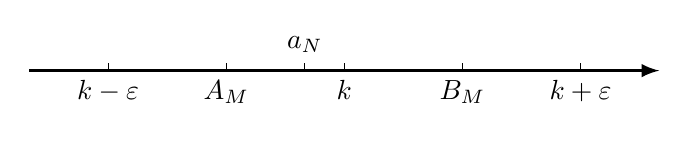
\begin{tikzpicture}[>=latex]
        \draw[very thick,->] (1,0)--(9,0);    
\foreach \x/\xtext in {5/k,2/k-\varepsilon,8/k+\varepsilon,3.5/A_M,6.5/B_M}
{
    \draw (\x,0)node[below]{$\xtext$}--(\x,.1);
}    
\draw (4.5,0)--(4.5,.1)node[above]{$a_N$};
    \end{tikzpicture}

    \caption{}
\end{figure}
\begin{equation}
    k-\varepsilon<A_M\le k\le B_M<k+\varepsilon
\end{equation}
由性质3知道,存在一个够大的$N$, 使得
\begin{equation}
    A_M<a_N    
\end{equation}
由性质2知道,$B_M$是一个上界,即恒有
\begin{equation}
    a_N\le B_M
\end{equation} 
由$\{a_n\}$的递增性,当$n\ge N$时,有
\begin{equation}
    a_N\le a_n
\end{equation} 
综合上述四点,就说明了当$n\ge N$时,有
\[k-\varepsilon<A_M\le a_N\le a_n<B_M<k+\varepsilon\]
亦即$|a_n-k|<\varepsilon$, 这也就说明了
$\Lim_{n\to\infty}a_n=k$。
\end{proof}








